\begin{figure}[htbp]
\centering
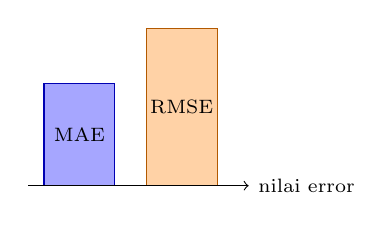
\begin{tikzpicture}[x=1cm,y=1cm]
  \draw[fill=blue!35, draw=blue!70!black] (0,0) rectangle (0.9,1.3)
    node[midway, font=\scriptsize, align=center] {MAE};
  \draw[fill=orange!35, draw=orange!70!black] (1.3,0) rectangle (2.2,2.0)
    node[midway, font=\scriptsize, align=center] {RMSE};
  \draw[->] (-0.2,0) -- (2.6,0) node[right, font=\scriptsize] {nilai error};
\end{tikzpicture}
\caption{Ilustrasi konseptual: pada outlier besar, RMSE cenderung lebih tinggi dari MAE karena kuadrat error; pilih metrik sesuai sensitivitas bisnis terhadap error ekstrem.}
\end{figure}
